\usepackage{tikz}
\usepackage{calc}
\usepackage{booktabs}
\usepackage{titlesec}
%\usepackage{hyperref}

% colors
\definecolor{color1}{HTML}{000060}
\definecolor{color1}{HTML}{C93AA4}
\definecolor{color2}{HTML}{666666}


% fonts
\usepackage{fontspec}
\defaultfontfeatures{Mapping=tex-text}
\setmainfont
[BoldFont=Lato-Bold.ttf,
ItalicFont=Lato-Italic.ttf,
BoldItalicFont=Lato-BoldItalic.ttf]
{Lato-Regular.ttf}
\newfontfamily\headingfont[ItalicFont=Lato-BlackItalic.ttf]{Lato-Black.ttf}
%%%

\usepackage{geometry}
\geometry{a4paper,
hmargin=20mm,vmargin=20mm,
head=0ex,foot=3ex}

\linespread{1.3}

\usepackage[hang]{caption}
\DeclareCaptionFormat{upper}{#1#2\uppercase{#3}\par}
\captionsetup{labelfont={bf,color=color2},textfont={small,color=color2},figurename=FIGURE,tablename=TABLE}

\titlespacing*{\section}
{0pt}{0ex}{7ex}

%%% fancy sections
\usepackage{titlesec}
%\titleformat{\chapter}{\headingfont\LARGE\bfseries\scshape\color{color1}}{\thechapter}{1em}{}[\titlerule]
\titleformat{\section}{\vspace*{20pt}\color{color1}\headingfont\Large\bfseries\uppercase}{\thesection}{1em}{}[\titlerule]
\titleformat{\subsection}{\color{color1}\headingfont\large\bfseries}{\thesubsection}{1em}{}
\titleformat{\subsubsection}{\color{color1}\headingfont\bfseries\uppercase}{\thesubsubsection}{1em}{}
%%%


% head and foot
\usepackage{fancyhdr}
\pagestyle{fancy}
\lhead{\color{color2}BEST EPICS IOC}
\chead{}
\makeatletter
\rhead{$
\begin{array}{l}

\includegraphics[height=15pt]{logo}
\end{array}$\color{color1}CAEN els s.r.l.
}
\makeatother
\newlength{\myheight}
\lfoot{
\settoheight{\myheight}{\thepage}
\raisebox{-2ex-0.5\myheight}{}
}
\cfoot{\color{color2}\thepage}
\rfoot{}
\renewcommand\headrulewidth{0.5pt}
\renewcommand\footrulewidth{0pt}

%%% picture on cover page
\usepackage{eso-pic}
\newcommand\BackgroundPic{%
\put(0,0){%
\parbox[b][\paperheight]{\paperwidth}{%
\vfill
\centering

\includegraphics[width=\paperwidth,height=\paperheight,%
keepaspectratio]{cover}%
\vfill
}}}
%%%
% custom titlepage
\makeatletter
\renewcommand{\maketitle}{
\thispagestyle{empty}
\AddToShipoutPicture*{\BackgroundPic}
\ClearShipoutPicture
%
\vfill
\phantom{a}
\medskip

\begin{center}
	$\begin{array}{l}    
\includegraphics[height=1.7cm]{logo_caenels_white} \end{array}$		
\end{center}
\vspace{30pt}

\vspace{100pt}


\begin{center}
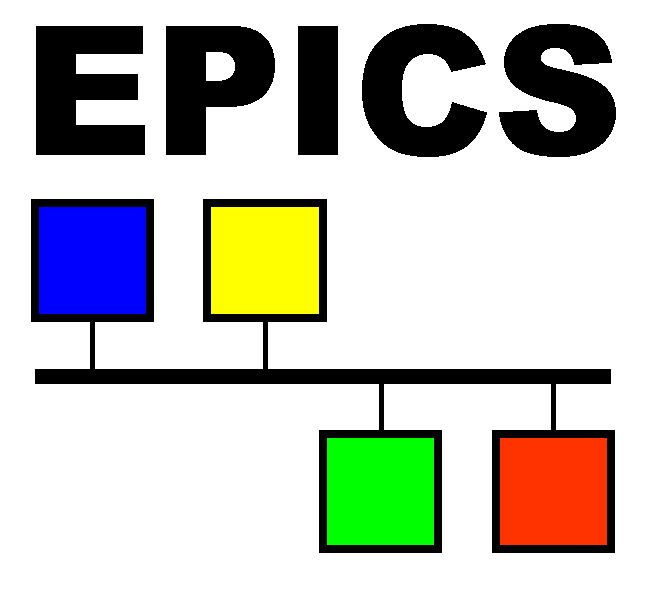
\includegraphics[width=150pt]{logo_659x595} 
	
\end{center}


\begin{center}
	
\end{center}
\vspace{30pt}
\begin{center}
	\begin{tabular}{c} %{@{}p{0.7\textwidth}@{}}
      \fontsize{30pt}{16pt}\selectfont\color{white}\headingfont\@title\\[50pt]
      \fontsize{20pt}{16pt}\selectfont\color{white}\headingfont\@subtitle\\[50pt]\\[50pt]
      \color{white}\headingfont\Large All rights reserved.\\[10pt]
      \color{white}\headingfont\Large\textcopyright \space  \@author
\end{tabular}
\end{center}
%
\clearpage
}
\makeatother
%%%


%%% fancy boxes

\usepackage{tcolorbox}
\usepackage{wrapfig}
\def\fullboxbegin{
\bigskip
\begin{tcolorbox}[colback=color1,colframe=color1,coltext=white,arc=0mm,boxrule=0pt]
}
\def\fullboxend{\end{tcolorbox}\medskip}
%
\def\leftboxbegin{
\begin{wrapfigure}{l}{0.4\textwidth}
\begin{tcolorbox}[colback=color1,colframe=color1,coltext=white,arc=0mm,boxrule=0pt]
}
\def\leftboxend{
\end{tcolorbox}
\end{wrapfigure}
}
%
\def\rightboxbegin{
\begin{wrapfigure}{r}{0.35\textwidth}
\begin{tcolorbox}[colback=color1,colframe=color1,coltext=white,arc=0mm,boxrule=0pt]
}
\def\rightboxend{
\end{tcolorbox}
\end{wrapfigure}
}
%
\newcounter{frames}
\def\frameboxbegin#1{
\bigskip
\refstepcounter{frames}
\begin{tcolorbox}[colback=color2,colframe=color1,arc=0mm,coltext=white,title={#1}]
}
\def\frameboxend{
\end{tcolorbox}
}

%\newcounter{frames}
%\def\frameboxbegin#1{
%	\bigskip
%	\refstepcounter{frames}
%	\begin{tcolorbox}[colback=white,colframe=color1,arc=0mm,title={\MakeUppercase{\textbf{Frame \arabic{frames}}: #1}}]
%	}
%	\def\frameboxend{
%	\end{tcolorbox}
%}

%%%